\documentclass[12pt]{article}

\usepackage[a4paper,margin=2.5cm]{geometry}
\usepackage{amsmath, amssymb, amsthm}
\usepackage{bm}
\usepackage{hyperref}
\usepackage{graphicx}
\usepackage{caption}
\usepackage{listings}
\usepackage{xcolor}
\usepackage{float}
\usepackage{placeins}
\graphicspath{{figures/}}

\lstdefinestyle{code}{
  basicstyle=\ttfamily\small,
  numbers=left,
  numberstyle=\tiny,
  numbersep=8pt,
  keywordstyle=\color{blue},
  commentstyle=\color{teal!70!black},
  stringstyle=\color{orange!70!black},
  showstringspaces=false,
  breaklines=true,
  frame=single,
  framerule=0.3pt,
  rulecolor=\color{black!15}
}
\lstset{style=code}

\title{Soft Actor-Critic (SAC) Tutorial}
\author{}
\date{\today}

\begin{document}
\maketitle

\section{Introduction}
Soft Actor-Critic (SAC) maximizes expected return while encouraging high-entropy policies. By combining stochastic policies with Q-function learning and automatic entropy tuning, SAC achieves state-of-the-art performance on continuous control benchmarks.

\section{Theory and Formulas}
\subsection{Maximum Entropy Objective}
SAC optimizes
\begin{equation}
J(\pi) = \mathbb{E}_{\tau \sim \pi}\Big[ \sum_{t} \gamma^t ( r_{t+1} + \alpha \mathcal{H}(\pi(\cdot\mid s_t)) ) \Big],
\end{equation}
where \(\alpha\) balances reward and entropy.

\subsection{Critic and Policy Updates}
Twin Q-functions \(Q_{w_i}\) minimize
\begin{equation}
L(w_i) = \mathbb{E}_{(s,a) \sim \mathcal{D}}\Big[ (Q_{w_i}(s,a) - y)^2 \Big], \quad y = r + \gamma (\min_j Q_{w_j^-}(s', a') - \alpha \log \pi_\theta(a'\mid s')).
\end{equation}
The policy is updated using the reparameterization trick:
\begin{equation}
\nabla_\theta J_{\pi} = \mathbb{E}_{s \sim \mathcal{D}, \varepsilon}\big[ \nabla_\theta \alpha \log \pi_\theta(f_\theta(\varepsilon; s)\mid s) - \nabla_\theta Q_{w_1}(s, f_\theta(\varepsilon; s)) \big].
\end{equation}

\subsection{Temperature Adaptation}
Entropy temperature \(\alpha\) is tuned by minimizing
\begin{equation}
J(\alpha) = \mathbb{E}_{a \sim \pi_\theta}\big[ -\alpha (\log \pi_\theta(a\mid s) + \mathcal{H}_{\text{target}}) \big].
\end{equation}
This keeps policy entropy near a target value, automating exploration-exploitation trade-offs.

\section{Applications and Tips}
\begin{itemize}
  \item \textbf{Continuous control}: locomotion, manipulation, autonomous driving.
  \item \textbf{Sample efficiency}: off-policy updates with replay buffers accelerate learning.
  \item \textbf{Robust policies}: entropy objective encourages diverse actions.
  \item \textbf{Best practices}: normalize observations, clip gradients, maintain twin critics, logarithmic parameterization for \(\alpha\), and monitor entropy as training progresses.
\end{itemize}

\section{Python Practice}
The script \texttt{gen\_sac\_figures.py} implements a lightweight SAC agent in a one-dimensional control environment. It records episode returns and the learned temperature across updates.
\begin{lstlisting}[language=Python,caption={Excerpt from gen_sac_figures.py}]
q_target = reward + gamma * (min_q_target - alpha * log_prob_next)
critic_w1 += critic_lr * (q_target - q1) * features(state, action)
critic_w2 += critic_lr * (q_target - q2) * features(state, action)

alpha_grad = -np.mean(log_prob + target_entropy)
log_alpha += alpha_lr * alpha_grad
alpha = np.exp(log_alpha)
\end{lstlisting}

\section{Result}
\begin{figure}[H]
  \centering
  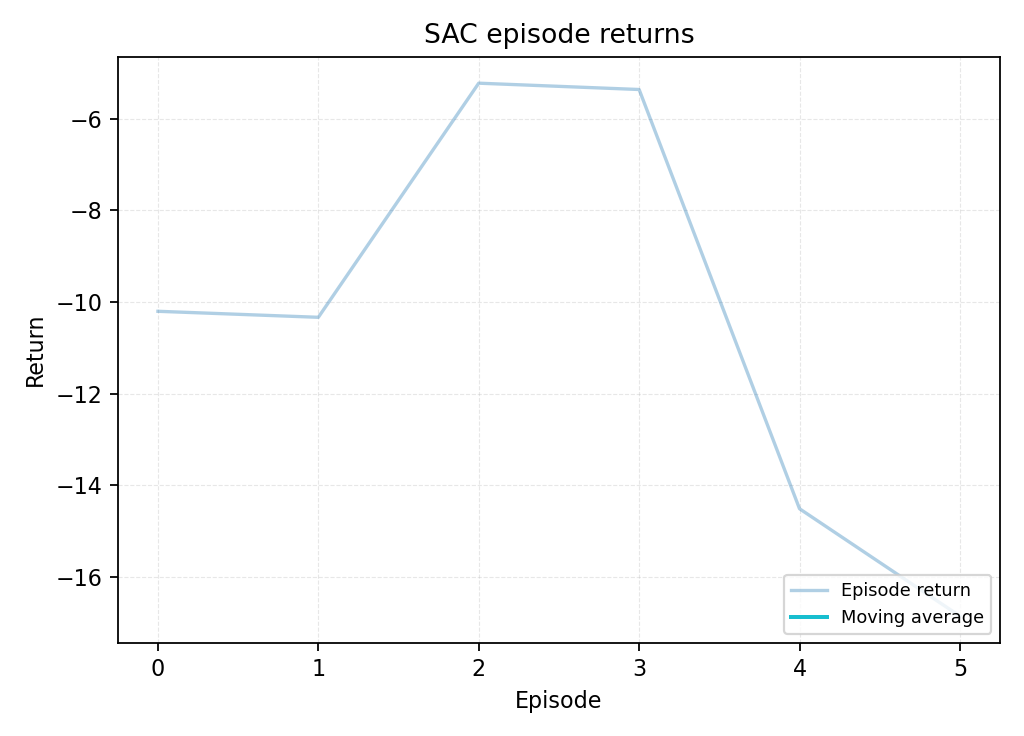
\includegraphics[width=0.8\linewidth]{sac_returns.png}
  \caption{SAC episode returns demonstrating stable improvement}
  \label{fig:sac_returns}
\end{figure}

\begin{figure}[H]
  \centering
  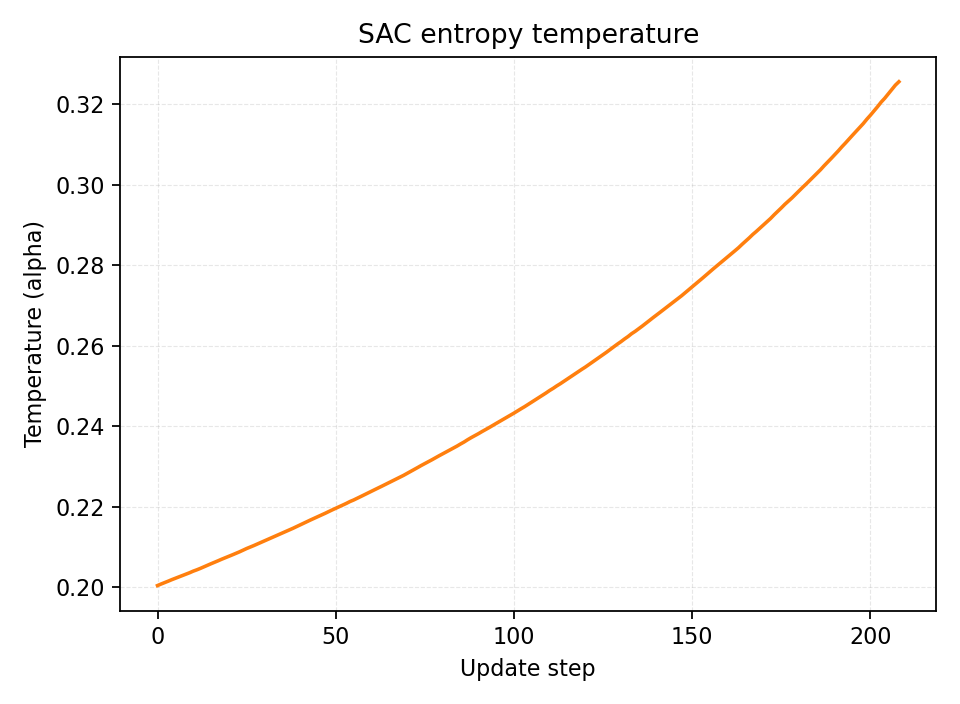
\includegraphics[width=0.82\linewidth]{sac_temperature.png}
  \caption{Entropy temperature trajectory approaching the target entropy}
  \label{fig:sac_temperature}
\end{figure}

\FloatBarrier
\section{Summary}
SAC maximizes reward and entropy simultaneously using twin Q-functions, stochastic actors, and automatic temperature tuning. Proper normalization, replay management, and entropy monitoring are essential. The toy control example illustrates increasing returns while the entropy temperature converges toward its target.

\end{document}